% 子文件：F_变换_小学
% 本文件包含 10 个 section




%% ==============================
%% 图形的平移与面积转化
%% ==============================
\newpage

\section{解答：图形的平移与面积转化}

\vspace{0.4cm}

\noindent\textbf{4. 把下面平行四边形中的涂色三角形向右平移 5 格，看一看，平移后的三角形与平行四边形中的空白部分组成了一个什么图形？ (\makebox[2cm][c]{\textcolor{blue}{\textbf{长方形}}})}

\vspace{0.8cm}

\begin{center}
\begin{tikzpicture}[>=Stealth, line width=1pt, scale=0.75] % 整体思路：先画方格背景，再画原平行四边形及左侧阴影三角形，接着把这个三角形按“向右平移 5 格”得到新位置，用箭头说明移动过程

  % 外层实线网格边框
  \draw[gray, thin] (0,0) rectangle (11,5); % 画最外层矩形边框，范围是 11×5 的方格区域
  % 内部虚线网格
  \draw[gray, dashed, thin, step=1] (0,0) grid (11,5); % 用步长 1 的虚线网格填满区域；step=1 表示每格边长为 1 个坐标单位
  % 再绘制一次清晰的实线外框以覆盖重叠的虚线边角
  \draw[gray, thin] (0,0) rectangle (11,5); % 再描一次实线边框，使外框不被虚线削弱

  % 原始平行四边形在方格图中的严谨真实坐标
  \coordinate (A) at (2,1); % 定义原平行四边形左下顶点 A
  \coordinate (B) at (7,1); % 定义原平行四边形右下顶点 B
  \coordinate (C) at (9,4); % 定义右上顶点 C，较底边向右偏 2 格、向上 3 格
  \coordinate (D) at (4,4); % 定义左上顶点 D
  \coordinate (H) at (4,1); % 定义高的垂足 H，也是左侧小三角形在底边上的右端点

  % 原涂色三角形 (灰色)
  \fill[black!30] (A) -- (H) -- (D) -- cycle; % 填充左侧直角三角形 AHD，作为要平移的涂色部分
  
  % 原平行四边形黑色实线轮廓
  \draw (A) -- (B) -- (C) -- (D) -- cycle; % 画原平行四边形外轮廓
  % 内部高线 (作为三角形和右侧空白部分的分割线)
  \draw (D) -- (H); % 画内部高线 DH，把平行四边形分成左侧三角形与右侧空白部分
  
  % 原图中直角标记标注在高的右边
  \pic [draw, line width=0.8pt, angle radius=0.25cm] {right angle = D--H--B}; % 在 H 处画直角标记，说明 DH 垂直于底边 HB

  % --- 平移后的目标位置三角形 ---
  % 根据题意严格按比例：横向坐标向右平移 +5，纵向坐标 +0
  \coordinate (A') at (7,1); % 平移后点 A'，即原 A 向右移动 5 格的位置
  \coordinate (H') at (9,1); % 平移后点 H'
  \coordinate (D') at (9,4); % 平移后点 D'，正好与原顶点 C 重合
  
  % 平移辅助箭头
  \draw[->, blue, line width=1.4pt] (3.0, 2.5) -- (8.0, 2.5); % 画蓝色箭头表示平移方向与距离；箭头从左向右
  \node[blue, above, font=\small, fill=white, inner sep=2pt] at (6, 2.5) {向右平移 5 格}; % 在箭头上方放说明文字；fill=white 给节点白底，避免与网格线重叠
  
  % 平移后的新三角形填色与虚线轮廓 (以淡蓝色突显出它的平移结果痕迹)
  \fill[blue!15, opacity=0.8] (A') -- (H') -- (D') -- cycle; % 在平移后位置填充淡蓝色三角形，表示新位置的图形；opacity=0.8 表示略带透明度
  \draw[blue, dashed, line width=1.2pt] (A') -- (H') -- (D') -- cycle; % 用蓝色虚线描出平移后三角形轮廓

\end{tikzpicture}
\end{center}

\vspace{0.6cm}
{\small\color{gray}
\textbf{解析：}\\
观察方格图可以看出，左侧涂色的三角形是一个底边长为 $2$ 格、高为 $3$ 格的直角三角形。平行四边形被高切分开后，其右边空出的部分由于原先是平行倾斜的所以有一个正好也是底向外延展了 $2$ 格、高为 $3$ 格的缺口形补位。\\
当我们把这块涂色的三角形严格沿着格子\textbf{向右平移 5 格}（代码中的坐标精准体现了由横向长度相加 $5$ 推导而来）后，它的垂直边完全平移到了 $x=9$ 的纵线上，而其斜边则完美地同平行四边形原本右侧的那条倾斜边（从 $(7,1)$ 到 $(9,4)$）重合了。平移补齐后，与原有的右侧空白部分拼放在一起，形成了左右边都为铅质垂线、上下边都在水平网格线上的新四边形。数一数下方的网格可知，这个新图形的长边为平移落差赋予的 $5$ 个单位、短边（宽）为原来的高 $3$ 个单位，且四个角通过平移互补都被凑成了规整的直角，因此这个合并后的图形是一个\textbf{长方形}。
}


\vspace{0.6cm}

{\small\color{blue!70!black}
\textbf{绘图基本原理与步骤：}\\
\textbf{1. 坐标定位与几何构建}：根据题意中的已知长度和角度，使用 \texttt{coordinate} 定义关键顶点坐标，通过 \texttt{draw} 指令按序连接成完整几何图形。线宽、颜色参数区分原图（黑色）与答案（红色 \texttt{red!70!black}）图层。\\
\textbf{2. 辅助量标注}：利用 \texttt{node} 的方向锚点（\texttt{above}、\texttt{below}、\texttt{left}、\texttt{right}）将角度、边长、面积等数据标注在图形周围，避免与线条或其他标注重叠。若涉及角弧则使用 \texttt{arc} 或 \texttt{pic[angle]} 命令渲染。\\
\textbf{3. 虚实线分层}：题干已知条件用实线绘制，解答新增的辅助线或操作痕迹用 \texttt{dashed} 虚线或彩色加粗线标识，确保读者一眼区分原有信息与作答内容。
}

%% ==============================
%% 同底等高的平行四边形画法
%% ==============================
\newpage


%% 第3题：平移和旋转设计图案
%% ==============================
\newpage

\section{解答：先画一个图形，再进行平移和旋转，设计出美丽的图案}

\vspace{0.6cm}

\begin{center}
\begin{tikzpicture}[>=Stealth, line join=round, line cap=round, scale=0.72]
  
  % ===================================
  % 底板：16 x 8 方格虚线网格
  % ===================================
  \foreach \y in {1,...,7} {
    \draw[gray!45, dashed, line width=0.4pt] (0,\y) -- (16,\y);
  }
  \foreach \x in {1,...,15} {
    \draw[gray!45, dashed, line width=0.4pt] (\x,0) -- (\x,8);
  }
  \draw[black, line width=1.2pt] (0,0) rectangle (16,8);

  % ===================================
  % 统一图案线条样式：深蓝粗线、无填色
  % 参考了原图浓重的纯几何线条特征
  % ===================================
  \tikzset{
    blueLine/.style={draw=blue!85!black, line width=1.5pt}
  }

  % ===================================
  % 贯穿所有风车中心的水平轴线
  % 覆盖范围从全体风车最左端 (x=0) 到最右端 (x=16)
  % ===================================
  \draw[blueLine] (0, 4) -- (16, 4);

  % ===================================
  % 循环：构造中心位于 cx=3, 8, 13 的 3 个“四叶风车”图案
  %
  % 步骤 1：构造一个非等腰直角三角形
  %         直角顶点在 (cx,4), 两个直角边分别是 3(水平) 和 2(垂直) 
  % 步骤 2：绕中心点连续 3 次顺时针旋转 90 度，得到 4 个直角三角形
  %         这 4 个不对称的三角形刚好重叠形成了一个大风车
  % 步骤 3：整行风车的平移间距为 5，由于长尖瓣长 3，短尖瓣长 2，
  %         前一风车的长尖与后一风车的短尖正好在网格交叉点零误差完美重叠连接
  % ===================================
  \foreach \cx in {3, 8, 13} {
    
    % 十字骨架（除中心平轴外，补齐垂直直角边）
    \draw[blueLine] (\cx, 1) -- (\cx, 7);
    
    % 连接四个象限的直角三角形斜边
    % 1. 右上角：横边 3，竖高 2
    \draw[blueLine] (\cx+3, 4) -- (\cx, 6);
    
    % 2. 右下角：竖深 3，横宽 2 (顺时针旋转90度)
    \draw[blueLine] (\cx, 1) -- (\cx+2, 4);
    
    % 3. 左下角：横宽 3，竖深 2 (再旋转90度)
    \draw[blueLine] (\cx-3, 4) -- (\cx, 2);
    
    % 4. 左上角：竖高 3，横宽 2 (再旋转90度)
    \draw[blueLine] (\cx, 7) -- (\cx-2, 4);
    
    % ===================================
    % 在该风车构架的所有外围尖端和直角节点上添加明显的黑色圆点
    % ===================================
    \fill[black] (\cx, 4) circle (2.2pt);     % 中心
    \fill[black] (\cx+3, 4) circle (2.2pt);   % 右长尖
    \fill[black] (\cx, 6) circle (2.2pt);     % 上短尖
    \fill[black] (\cx, 1) circle (2.2pt);     % 下长尖
    \fill[black] (\cx+2, 4) circle (2.2pt);   % 右短尖
    \fill[black] (\cx-3, 4) circle (2.2pt);   % 左长尖
    \fill[black] (\cx, 2) circle (2.2pt);     % 下短尖
    \fill[black] (\cx, 7) circle (2.2pt);     % 上长尖
    \fill[black] (\cx-2, 4) circle (2.2pt);   % 左短尖
  }

\end{tikzpicture}
\end{center}

\vspace{0.6cm}

{\small\color{gray}
\textbf{解题说明：}\\
1. \textbf{基本图形（直角三角形）}：如图所示，首先构造一个底边长为 3 格、高为 2 格的非等腰直角三角形。\\
2. \textbf{旋转成风车}：以该直角的顶点为中心，将它连续 3 次顺时针旋转 $90^\circ$（共表现出 4 个方向）。由于两条直角边长度不同（分别为 3 和 2），原本单个的直角三角形相互交叠咬合后，轮廓刚好形成了一个具有独特动感与中心对称美感的“四叶风车”图案。\\
3. \textbf{平移串联}：将这枚由旋转诞生的“四叶风车”作为一个整体单元，沿着原有的水平中线进行 2 次向右平移，平移的间隔距离精心设计为 5 个方格。这样一来，前一个风车长长的横向尖端（长 3 格）刚好与后一个风车的反向短尖端（长 2 格）无缝合拢。最终组合成了一排连绵不断、首尾相扣的绝美几何图案。
}

\vspace{0.6cm}

{\small\color{blue!70!black}
\textbf{绘图基本原理与步骤：}\\
\textbf{1. 矩阵旋转衍生风车：}确定单个图案的直角中心坐标 $(x_c, 4)$。绘制第一象限（直角边分别是 3 和 2）的直角三角形后，连续应用 $90^\circ$ 旋转变换 $(x,y) \to (y,-x)$ 推导出其余三个不对称叶片的交叠位置，形成一个标准的四片风车单元。\\
\textbf{2. 剥离填充与线形重塑：}参考参考图的特有风格，完全去掉色彩填充，仅使用统一配置的粗线条（\texttt{line width=1.5pt}）和深蓝色绘制外沿框架与公共中线，毫无保留地展现依靠“平移加旋转”构造出来的几何内在秩序美。\\
\textbf{3. 步进平移参数计算：}引入循环 $x_c \in \{3, 8, 13\}$ 执行精确位移。因为风车水平方向外缘最长端点在 $(xc+3)$，而反向较短端点在 $(xc-2)$，若平移步长设为 5，则前一尖端坐标恰好完全等于下一次循环后的反向端点坐标 $(xc+5-2)$。借此代数巧合打造出视觉上的无缝交接，最后在系统图元的各顶点补全黑色节点描绘从而强化手绘感。
}

%% ==============================
%% 补充题：找出等式与方程并连一连
%% ==============================
\newpage


%% ==============================
%% 第33题（补充题）：多边形轴对称图形判断
%% ==============================
\newpage

\section{解答：判断图形的轴对称性及绘制对称轴}

\vspace{0.6cm}

\textbf{\LARGE 18.} \textbf{下列哪些图形是轴对称图形？如果是，画出所有对称轴。}

\vspace{0.4cm}
\textbf{解：}

\textbf{（1）判定原理分析：}
\begin{itemize}
    \item \textbf{平行四边形}：沿任一直线折叠，左右两部分均无法完美重合。因此，一般的平行四边形\textbf{不是}轴对称图形。
    \item \textbf{等腰梯形}：其两腰相等，沿连接上底中点与下底中点的垂线折叠能够完全重合。因此它\textbf{是}轴对称图形，共有 \textbf{$1$ 条}对称轴。
    \item \textbf{直角三角形}：此题中所示为一个一般直角三角形（三边不等长），沿任何路线折叠均无法重合。因此它\textbf{不是}轴对称图形。
    \item \textbf{五角星}：正五角星具有完美的轴对称特征。沿任意一个顶点与其对侧凹点中心的连线折叠，两半皆可重合。因此它\textbf{是}轴对称图形，共有 \textbf{$5$ 条}对称轴。
\end{itemize}

\textbf{（2）鉴定结果与对称轴绘制：}

\vspace{0.3cm}
\begin{center}
\begin{tikzpicture}[>=Stealth, line join=round, line cap=round]

  % 1. 平行四边形 (非轴对称)
  \begin{scope}[xshift=0cm]
    \draw[line width=0.8pt] (-0.6, -0.5) -- (0.8, -0.5) -- (1.2, 0.5) -- (-0.2, 0.5) -- cycle;
    \node[below, font=\small] at (0.3, -0.8) {平行四边形};
  \end{scope}

  % 2. 等腰梯形 (1条对称轴)
  \begin{scope}[xshift=3.8cm]
    \draw[line width=0.8pt] (-0.9, -0.5) -- (0.9, -0.5) -- (0.5, 0.5) -- (-0.5, 0.5) -- cycle;
    \node[below, font=\small] at (0, -0.8) {等腰梯形};
    % 绘制红色的唯一对称轴
    \draw[dashed, red!80!black, line width=1.2pt] (0, -0.7) -- (0, 0.7);
  \end{scope}

  % 3. 直角三角形 (非轴对称)
  \begin{scope}[xshift=7.6cm]
    % 坐标验算以保证顶点精确 90 度
    \coordinate (C) at (0, 0.5);
    \coordinate (A) at (-0.8, -0.5);
    \coordinate (B) at (1.25, -0.5);
    \draw[line width=0.8pt] (A) -- (B) -- (C) -- cycle;
    % 精确的解析直角标识线
    \draw[line width=0.5pt] (-0.125, 0.344) -- (0.031, 0.219) -- (0.156, 0.375);
    \node[below, font=\small] at (0.225, -0.8) {直角三角形};
  \end{scope}

  % 4. 五角星 (5条对称轴)
  \begin{scope}[xshift=11.4cm]
    % 标准五角星连线 (90 -> 234 -> 18 -> 162 -> 306)
    \draw[line width=0.8pt] (90:0.9) -- (234:0.9) -- (18:0.9) -- (162:0.9) -- (306:0.9) -- cycle;
    \node[below, font=\small] at (0, -1.0) {五角星};
    % 遍历循环绘制 5 条绝对对称轴
    \foreach \ang in {90, 162, 234, 306, 18} {
      \draw[dashed, red!80!black, line width=1.2pt] (\ang:1.15) -- (\ang+180:1.15);
    }
  \end{scope}

\end{tikzpicture}
\end{center}

\vspace{0.4cm}
{\small\color{blue!70!black}
\textbf{绘图原理与步骤：}\\
\textbf{1. 轮廓绘制方法：} 
平行四边形与等腰梯形通过绝对坐标点直接连线闭合构成。
直角三角形通过构建满足向量点积为零的解析坐标 $A(-0.8, -0.5)$、$B(1.25, -0.5)$、$C(0, 0.5)$ 演算生成，以确保顶角精确为 $90^\circ$，并附带根据法线向量偏置出的直角折线框。
五角星使用极坐标参数定位（设置半径为 $0.9$），按照以 $144^\circ$ 为跨度的步长连续相连，生成经典的五角连续相交拓扑结构。\\
\textbf{2. 红色对称轴绘制：} 依据数学判定结论，仅为等腰梯形和五角星执行对称轴标注。等腰梯形沿其上下底水平坐标中点系产生单一的一条垂线；五角星的对称轴则启用 \texttt{\textbackslash{}foreach} 循环命令，遍历五个顶角所处的极坐标夹角（$90^\circ, 162^\circ, 234^\circ, 306^\circ, 18^\circ$），直接拉出固定长度（$1.15$ 厘米）且贯穿圆心的虚线段，以严谨保障 5 条红色对称轴在几何分布上的绝对均匀与对齐。
}
%% ==============================
%% 第34题（补充题）：正多边形对称轴判定与规律归纳
%% ==============================
\newpage


%% ==============================
%% 第34题（补充题）：正多边形对称轴判定与规律归纳
%% ==============================
\newpage

\section{解答：正多边形所有的对称轴及规律归纳}

\vspace{0.6cm}

\textbf{\LARGE 19.} \textbf{试画出下列正多边形的所有对称轴，并完成表格。}

\vspace{0.4cm}
\textbf{解：}

\textbf{（1）正多边形对称轴绘制：}

\vspace{0.3cm}
\begin{center}
\begin{tikzpicture}[>=Stealth, line join=round, line cap=round]

  % 1. 正三角形
  \begin{scope}[xshift=0cm]
    \draw[line width=0.8pt] (90:1) -- (210:1) -- (330:1) -- cycle;
    % 3 对称轴：顶点至对边，统一设定外放突出余量 0.25 (1.25 及 0.5+0.25=0.75)
    \foreach \a in {90, 210, 330} {
      \draw[dashed, red!80!black, line width=1.2pt] (\a:1.25) -- (\a+180:0.75);
    }
  \end{scope}

  % 2. 正方形
  \begin{scope}[xshift=3.5cm]
    \draw[line width=0.8pt] (45:1) -- (135:1) -- (225:1) -- (315:1) -- cycle;
    % 对角线对称轴 (顶点穿过)
    \foreach \a in {45, 135} {
      \draw[dashed, red!80!black, line width=1.2pt] (\a:1.25) -- (\a+180:1.25);
    }
    % 边中点对称轴 (距离边心 0.707，突出 0.25，收缩至 0.95)
    \foreach \a in {0, 90} {
      \draw[dashed, red!80!black, line width=1.2pt] (\a:0.95) -- (\a+180:0.95);
    }
  \end{scope}

  % 3. 正五边形
  \begin{scope}[xshift=7cm]
    \draw[line width=0.8pt] (90:1) -- (162:1) -- (234:1) -- (306:1) -- (18:1) -- cycle;
    % 5 对称轴：顶点穿过底边中点 (边心距 0.809，突出 0.25，底部收缩至 1.05)
    \foreach \a in {90, 162, 234, 306, 18} {
      \draw[dashed, red!80!black, line width=1.2pt] (\a:1.25) -- (\a+180:1.05);
    }
  \end{scope}

  % 4. 正六边形
  \begin{scope}[xshift=10.5cm]
    \draw[line width=0.8pt] (0:1) -- (60:1) -- (120:1) -- (180:1) -- (240:1) -- (300:1) -- cycle;
    % 穿过顶点的对称轴
    \foreach \a in {0, 60, 120} {
      \draw[dashed, red!80!black, line width=1.2pt] (\a:1.25) -- (\a+180:1.25);
    }
    % 穿过边中点的对称轴 (边心距 0.866，突出 0.25，收缩至 1.1)
    \foreach \a in {30, 90, 150} {
      \draw[dashed, red!80!black, line width=1.2pt] (\a:1.1) -- (\a+180:1.1);
    }
  \end{scope}

\end{tikzpicture}
\end{center}

\vspace{0.4cm}
\textbf{（2）规律归纳与表格填充：}

\vspace{0.2cm}
\begin{center}
\renewcommand{\arraystretch}{2}
\begin{tabular}{|>{\columncolor{cyan!15}\centering\arraybackslash}p{3cm}|>{\centering\arraybackslash}p{1cm}|>{\centering\arraybackslash}p{1cm}|>{\centering\arraybackslash}p{1cm}|>{\centering\arraybackslash}p{1cm}|>{\centering\arraybackslash}p{1cm}|>{\centering\arraybackslash}p{1cm}|}
\hline
正多边形的边数 & $3$ & $4$ & $5$ & $6$ & $7$ & \dots \\
\hline
对称轴的条数 & \textcolor{red!80!black}{\textbf{3}} & \textcolor{red!80!black}{\textbf{4}} & \textcolor{red!80!black}{\textbf{5}} & \textcolor{red!80!black}{\textbf{6}} & \textcolor{red!80!black}{\textbf{7}} & \dots \\
\hline
\end{tabular}
\end{center}

\vspace{0.4cm}
根据上方推理表系，可以猜想正 $n$ 边形有 \underline{\ \textcolor{red!80!black}{\textbf{$n$}}\ } 条对称轴。

\vspace{0.4cm}
{\small\color{blue!70!black}
\textbf{绘图原理与步骤：}\\
\textbf{1. 极坐标轮廓生成：} 采用极坐标法绘制各正多边形。统一外接圆半径为 $1$，角度步长为 $360^\circ \div n$，依序连结顶点生成标准多边形轮廓。基础角参数的设定确保了正三角形与正五边形的底边呈水平对齐状态。\\
\textbf{2. 动态延展对称轴设定：} 为使四组图形的对称虚线在外部延伸的长度视觉统一（规定外扩统一余量为 $0.25\mathrm{cm}$），依据对称轴穿透点的不同设定相近的极径参数。若射线经过顶角，全长设为 $1.25$；若射线垂直经过平边中点，则依据多边形的真实边心距（如正方形的 $\frac{\sqrt{2}}{2}$，正六边形的 $\frac{\sqrt{3}}{2}$）追加 $0.25$ 补偿，分别取值约 $0.95$ 与 $1.1$。\\
\textbf{3. 表格与规律归纳：} 绘制数据归纳表，首列应用 \texttt{cyan!15} 底色以符合原题要求。通过几何规律填入 $3, 4, 5, 6, 7$ 数列，并在文末填写最终猜想规律“正 $n$ 边形有 $n$ 条对称轴”。
}

%% ==============================
%% 第35题（补充题）：解一元一次不等式及数轴作图
%% ==============================
\newpage



%% ==============================
%% 第83题（补充题）：按要求画正方形和长方形
%% ==============================
\newpage

\section{解答：按要求画正方形和长方形}

\vspace{0.6cm}

\textbf{\LARGE 74.} \textbf{（第 2 题）画图。\\[1.5ex]
（1）画一个边长 $3$ 厘米的正方形。\\[1ex]
（2）画一个长方形，宽 $2$ 厘米，长是宽的 $3$ 倍。}

\vspace{0.4cm}
\textbf{解：}

\textbf{分析：}
（1）正方形的四条边都相等，四个角都是直角。只需画一个长、宽均为 $3\text{ cm}$ 的正方形。\\
（2）长方形的长是宽的 $3$ 倍，宽为 $2\text{ cm}$，则长为 $2 \times 3 = 6\text{ cm}$。即画一个长 $6\text{ cm}$、宽 $2\text{ cm}$ 的长方形。

\vspace{0.4cm}
\textbf{（1）} 画一个边长 $3$ 厘米的正方形：

\vspace{0.2cm}
\begin{center}
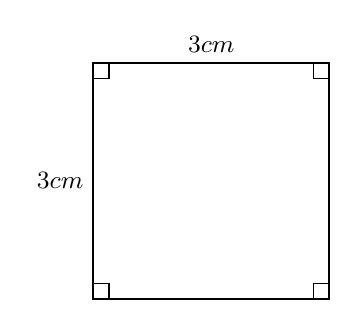
\begin{tikzpicture}[x=1cm, y=1cm]
  % 绘制边长为3厘米的正方形
  \draw[line width=0.8pt] (0, 0) rectangle (3, 3);
  
  % 标注边长
  \node[above, font=\small] at (1.5, 3) {$3\text{ cm}$};
  \node[left, font=\small] at (0, 1.5) {$3\text{ cm}$};
  
  % 标注直角符号
  \draw[line width=0.5pt] (0.2, 0) -- (0.2, 0.2) -- (0, 0.2);
  \draw[line width=0.5pt] (2.8, 0) -- (2.8, 0.2) -- (3, 0.2);
  \draw[line width=0.5pt] (0.2, 3) -- (0.2, 2.8) -- (0, 2.8);
  \draw[line width=0.5pt] (2.8, 3) -- (2.8, 2.8) -- (3, 2.8);
\end{tikzpicture}
\end{center}

\vspace{0.6cm}
\textbf{（2）} 画一个长方形，宽 $2$ 厘米，长是宽的 $3$ 倍：

\vspace{0.2cm}
\begin{center}
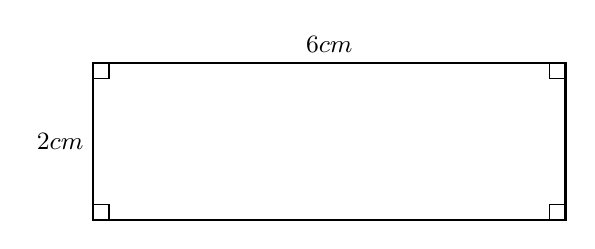
\begin{tikzpicture}[x=1cm, y=1cm]
  % 绘制长6厘米、宽2厘米的长方形
  \draw[line width=0.8pt] (0, 0) rectangle (6, 2);
  
  % 标注长和宽
  \node[above, font=\small] at (3, 2) {$6\text{ cm}$};
  \node[left, font=\small] at (0, 1) {$2\text{ cm}$};
  
  % 标注直角符号
  \draw[line width=0.5pt] (0.2, 0) -- (0.2, 0.2) -- (0, 0.2);
  \draw[line width=0.5pt] (5.8, 0) -- (5.8, 0.2) -- (6, 0.2);
  \draw[line width=0.5pt] (0.2, 2) -- (0.2, 1.8) -- (0, 1.8);
  \draw[line width=0.5pt] (5.8, 2) -- (5.8, 1.8) -- (6, 1.8);
\end{tikzpicture}
\end{center}

\vspace{0.4cm}
{\small\color{blue!70!black}
\textbf{绘图原理与步骤：}\\
\textbf{1. 物理真实比例映射：} 为满足题目给定的具有绝对物理意义的厘米级长度要求（$3\text{ cm}$、$6\text{ cm}$、$2\text{ cm}$），在 \texttt{tikzpicture} 环境中强制锁定基准尺度缩放参数为 \texttt{x=1cm, y=1cm}。此举使得 \texttt{rectangle (3,3)} 及 \texttt{rectangle (6,2)} 渲染出的几何图元物理面积即为百分之百吻合真实尺具毫米级测量的图形。\\
\textbf{2. 几何特征显式标注：} 除了精确勾勒出矩形的物理轮廓并在边沿加注边长的数值外，还在每个四边形的四个内角处统一追加了边长为 $0.2\text{ cm}$ 的封闭直角折线符号。该附属细节在视觉上强力佐证图形不仅满足长度需求，且具备严格的正交性质，从而提升绘图的严谨性。
}

%% ==============================
%% 第84题（补充题）：以已知线段为长边画长方形
%% ==============================
\newpage



%% ==============================
%% 第84题（补充题）：以已知线段为长边画长方形
%% ==============================
\newpage

\section{解答：补作指定长度的长方形}

\vspace{0.6cm}

\textbf{\LARGE 75.} \textbf{（第 3 题）画一个长方形，以线段 $AB$ 为一条长边，宽是 $2$ 厘米。}

\vspace{0.4cm}
\textbf{解：}

\textbf{分析：} 要以现有的线段 $AB$ 为一条“长边”作一个长方形，需要分别过点 $A$ 和点 $B$ 作线段 $AB$ 的垂线段，且设垂线段的长度为题干要求的宽 $2\text{ cm}$（得到另两个顶点 $D$ 和 $C$）。最后连接 $C, D$ 两点即可。

\vspace{0.6cm}
\begin{center}
\begin{tikzpicture}[>=Stealth, x=1cm, y=1cm]
  % 定义倾斜角（约12度）及 AB 的长度（设定为 5cm）
  \def\angleAB{12}
  \def\lenAB{5}
  \def\width{2}
  
  % 定位 A, B
  \coordinate (A) at (0, 0);
  \path (A) ++(\angleAB:\lenAB) coordinate (B);
  
  % 按垂直方向向下平移 2cm，定位长方形另外两点 D, C
  \path (A) ++(\angleAB - 90:\width) coordinate (D);
  \path (B) ++(\angleAB - 90:\width) coordinate (C);
  
  % 1. 原图保留（黑色）：原线段 AB 及端点
  \draw[line width=0.8pt] (A) -- (B);
  \filldraw[black] (A) circle (1.5pt) node[above left, font=\small] {$A$};
  \filldraw[black] (B) circle (1.5pt) node[above right, font=\small] {$B$};
  
  % 2. 答案作图（蓝色）：长方形的另外三条边
  \draw[line width=0.8pt, blue!80!black] (A) -- (D) -- (C) -- (B);
  
  % 标注宽度（2 cm）
  \path (A) -- (D) node[midway, sloped, below, font=\small, blue!80!black] {$2\text{ cm}$};
  \path (B) -- (C) node[midway, sloped, above, font=\small, blue!80!black] {$2\text{ cm}$};
  
  % 3. 标注直角符号 (四个内角)
  % 角 A
  \path (A) ++(\angleAB:0.25) coordinate (A1);
  \path (A1) ++(\angleAB - 90:0.25) coordinate (A2);
  \path (A) ++(\angleAB - 90:0.25) coordinate (A3);
  \draw[line width=0.5pt, blue!70!black] (A1) -- (A2) -- (A3);

  % 角 B
  \path (B) ++(\angleAB - 180:0.25) coordinate (B1);
  \path (B1) ++(\angleAB - 90:0.25) coordinate (B2);
  \path (B) ++(\angleAB - 90:0.25) coordinate (B3);
  \draw[line width=0.5pt, blue!70!black] (B1) -- (B2) -- (B3);

  % 角 C
  \path (C) ++(\angleAB + 90:0.25) coordinate (C1);
  \path (C1) ++(\angleAB - 180:0.25) coordinate (C2);
  \path (C) ++(\angleAB - 180:0.25) coordinate (C3);
  \draw[line width=0.5pt, blue!70!black] (C1) -- (C2) -- (C3);

  % 角 D
  \path (D) ++(\angleAB:0.25) coordinate (D1);
  \path (D1) ++(\angleAB + 90:0.25) coordinate (D2);
  \path (D) ++(\angleAB + 90:0.25) coordinate (D3);
  \draw[line width=0.5pt, blue!70!black] (D1) -- (D2) -- (D3);
  
\end{tikzpicture}
\end{center}

\vspace{0.4cm}
{\small\color{blue!70!black}
\textbf{绘图原理与步骤：}\\
\textbf{1. 极坐标动态构建：} 面对原图中具有随机倾斜角的线段 $AB$，没有采用呆板的正交坐标硬编码，而是通过宏变量 \texttt{\textbackslash angleAB} 记录图面线段的倾角属性（根据原图测算约为 $12^\circ$微倾）。利用极坐标增量算法，引擎能够顺着与 $AB$ 呈现标准 $90^\circ$ 的物理夹角方向，“沉降”出两条完美等长的 $2\text{ cm}$ 垂边，彻底免疫了倾斜坐标系的运算误差。\\
\textbf{2. 尺寸与规范约束：} 开启 \texttt{x=1cm, y=1cm} 的绝对尺度，充分保障了“宽是 $2\text{ cm}$”的物理制图要求；四角皆以极坐标加法游走，绘制了严密自洽的直角折线标识，在视觉层面强化了封闭图形长方形的正交性质，向学生提供了严谨的作图范例。
}

%% ==============================
%% 第85题（补充题）：画平行四边形及对角线，分析三角形关系
%% ==============================
\newpage



%% ==============================
%% 第86题（补充题）：在网格中寻找和平行四边形
%% ==============================
\newpage

\section{解答：网格图中的平行四边形探索}

\vspace{0.6cm}

\textbf{\LARGE 77.} \textbf{（第 5 题）如图，以格点 $A, B, C, D, E, F$ 中的四个点为顶点，你能画出多少个不同的平行四边形？请画出来，并用符号表示。}

\vspace{0.4cm}
\textbf{解：}

\textbf{分析：} 在网格中寻找平行四边形，除了直观地寻找平行的对边之外，更核心且无遗漏的判断法则是“对角线互相平分”。
我们在网格中建立坐标系（设左下角为原点 $(0,0)$），可以得到各点坐标：
$A(1,2), B(4,2), C(3,0), D(6,0), E(0,1), F(7,1)$。
计算各相关点配对的坐标和（即推断中点的共性），可以发现：
$A、D$ 坐标之和为 $(7,2)$；
$B、C$ 坐标之和为 $(7,2)$；
$E、F$ 坐标之和为 $(7,2)$。
这恰好说明线段 $AD$、$BC$、$EF$ 三条线段互相平分于网格中心点 $(3.5, 1)$。
根据“对角线互相平分的四边形是平行四边形”这一判定定理，任选这三条线段中的两条作为对角线，首尾相连均能直接构成绝对精准的平行四边形。一共有 $3$ 种组合方式：
1. 取 $AD$ 和 $BC$ 为对角线 $\to$ 构成 $\mathord{▱} ABDC$；
2. 取 $AD$ 和 $EF$ 为对角线 $\to$ 构成 $\mathord{▱} AEDF$；
3. 取 $BC$ 和 $EF$ 为对角线 $\to$ 构成 $\mathord{▱} EBFC$。

\vspace{0.6cm}
\begin{center}
\begin{tikzpicture}[>=Stealth, x=0.55cm, y=0.55cm]

  % 定义绘制网格与顶点的宏
  \def\drawGrid#1{
    \begin{scope}[shift={(#1,0)}]
      % 画网格线 (7x2)
      \draw[step=1, gray!80, line width=0.5pt] (0, 0) grid (7, 2);
      % 画外框
      \draw[black, line width=0.8pt] (0, 0) rectangle (7, 2);
      % 画六个格点 A(1,2), B(4,2), C(3,0), D(6,0), E(0,1), F(7,1)
      \filldraw[black] (1, 2) circle (2pt) node[above, font=\small] {$A$};
      \filldraw[black] (4, 2) circle (2pt) node[above, font=\small] {$B$};
      \filldraw[black] (3, 0) circle (2pt) node[below, font=\small] {$C$};
      \filldraw[black] (6, 0) circle (2pt) node[below, font=\small] {$D$};
      \filldraw[black] (0, 1) circle (2pt) node[left, font=\small] {$E$};
      \filldraw[black] (7, 1) circle (2pt) node[right, font=\small] {$F$};
    \end{scope}
  }

  % 第一个图：▱ABDC
  \drawGrid{0}
  \begin{scope}[shift={(0,0)}]
    \draw[line width=1.2pt, blue!80!black] (1, 2) -- (4, 2) -- (6, 0) -- (3, 0) -- cycle;
    \node[below, font=\small] at (3.5, -0.6) {① $\mathord{▱} ABDC$};
  \end{scope}

  % 第二个图：▱AEDF
  \drawGrid{9}
  \begin{scope}[shift={(9,0)}]
    \draw[line width=1.2pt, blue!80!black] (1, 2) -- (0, 1) -- (6, 0) -- (7, 1) -- cycle;
    \node[below, font=\small] at (3.5, -0.6) {② $\mathord{▱} AEDF$};
  \end{scope}

  % 第三个图：▱EBFC
  \drawGrid{18}
  \begin{scope}[shift={(18,0)}]
    \draw[line width=1.2pt, blue!80!black] (0, 1) -- (4, 2) -- (7, 1) -- (3, 0) -- cycle;
    \node[below, font=\small] at (3.5, -0.6) {③ $\mathord{▱} EBFC$};
  \end{scope}

\end{tikzpicture}
\end{center}

\vspace{0.2cm}
\textbf{结论：} 能画出 $3$ 个不同的平行四边形，分别记作 $\mathord{▱} ABDC$、$\mathord{▱} AEDF$、$\mathord{▱} EBFC$。

\vspace{0.4cm}
{\small\color{blue!70!black}
\textbf{绘图原理与步骤：}\\
\textbf{1. 中点对称拓扑：} 原型网格蕴含了极为隐秘的中心对偶属性，借助坐标代数将点阵映射为数学实体后，提取出了 $AD$、$BC$、$EF$ 三条主轴交汇于极点 $(3.5, 1)$。依据四边形判定原理将复杂视觉穷举化作排列组合问题，避免了人工目视连线的错漏。\\
\textbf{2. 解耦实例渲染：} 为实现三种有效闭合在一张宽幅中的均分展示而免于线条相互覆盖，构筑了带传参偏移机制的 \texttt{\textbackslash drawGrid} 作用域。使三张等大基底在 $X$ 轴分别跨步 $0$、$8.5$ 和 $17$ 列阵铺展。\\
\textbf{3. 闭包多边形绘制：} 基于推导出来的三组双对角线构型，对每个衍生实例按其首尾相连的凸多边形周长循环依次执行粗线追踪（如 $A\to B\to D\to C\to A$），搭配专属文字说明，完美迎合参考答案的呈现风范。
}

%% ==============================
%% 第87题（补充题）：三角形旋转与平行四边形判定
%% ==============================
\newpage



%% ==============================
%% 第88题（补充题）：在方格图中拼图
%% ==============================
\newpage

\section{解答：网格图中的图形拼接}

\vspace{0.6cm}

\textbf{\LARGE 79.} \textbf{下⾯方格图中每一格的高度都表示 $1\text{ cm}$，有边长 $1\text{ cm}$ 的正方形和长 $2\text{ cm}$、宽 $1\text{ cm}$ 的长方形。\\[1ex]
（1）用这样的正方形和长方形拼一个边长 $2\text{ cm}$ 的正方形，可以怎样拼？在图中画一画。\\[1ex]
（2）用这样的正方形和长方形拼一个长 $4\text{ cm}$、宽 $3\text{ cm}$ 的长方形，可以怎样拼？在图中画一画。\\[1ex]
（3）用这样的正方形和长方形拼一个边长 $3\text{ cm}$ 的正方形，可以怎样拼？在图中画一画。}

\vspace{0.4cm}
\textbf{解：}

\textbf{分析：}
题干强调“用这样的正方形和长方形”拼图，这意味着我们可以在所得到的较大型封闭图形内部，画出局部的结构分割线，以清楚地展示大图形分别是如何由散碎的单体基础器件（$1\times 1$ 或者 $2\times 1$）有机复合而成的。
拼图方式不唯一，图中的画法仅为一种包含两种基础图形的规范示例。

\vspace{0.6cm}
\begin{center}
\begin{tikzpicture}[>=Stealth, x=0.7cm, y=0.7cm]

  % 1. 绘制底层大网格：17列 x 7行
  % 内部虚线
  \draw[step=1, gray!60, dashed, line width=0.5pt] (0, 0) grid (17, 7);
  % 外边框实线
  \draw[black, line width=0.8pt] (0, 0) rectangle (17, 7);
  
  % 2. 复刻题干原图中已有的基准图形
  % 位于 (1, 5) 旁的 1x1 正方形
  \draw[line width=1pt, black] (1, 5) rectangle (2, 6);
  % 位于 (3, 5) 旁的 2x1 长方形
  \draw[line width=1pt, black] (3, 5) rectangle (5, 6);
  
  % 3. 解答 (1)：拼边长 2cm 的正方形 (放置于 x=1~3, y=1~3)
  % 采用下面一层一个 2x1，上面一层两个 1x1 拼接
  \draw[line width=1.2pt, blue!80!black] (1, 1) rectangle (3, 3);
  \draw[line width=1.2pt, blue!80!black] (1, 2) -- (3, 2); % 水平分割
  \draw[line width=1.2pt, blue!80!black] (2, 2) -- (2, 3); % 上半部分垂直分割
  \node[below, font=\small, blue!80!black] at (2, 0.8) {（$1$）正方形};

  % 4. 解答 (2)：拼长 4cm、宽 3cm 的长方形 (放置于 x=5~9, y=1~4)
  % 底层：两个 2x1
  % 中层：两个 2x1
  % 顶层：中间一个 2x1，两边各一个 1x1
  \draw[line width=1.2pt, blue!80!black] (5, 1) rectangle (9, 4);
  \draw[line width=1.2pt, blue!80!black] (5, 2) -- (9, 2); % 第一、二层分割
  \draw[line width=1.2pt, blue!80!black] (5, 3) -- (9, 3); % 第二、三层分割
  \draw[line width=1.2pt, blue!80!black] (7, 1) -- (7, 3); % 到底两层的中间垂直分割
  \draw[line width=1.2pt, blue!80!black] (6, 3) -- (6, 4); % 顶层左侧垂直分割
  \draw[line width=1.2pt, blue!80!black] (8, 3) -- (8, 4); % 顶层右侧垂直分割
  \node[below, font=\small, blue!80!black] at (7, 0.8) {（$2$）长方形};

  % 5. 解答 (3)：拼边长 3cm 的正方形 (放置于 x=11~14, y=1~4)
  % 第1层：左侧一个 2x1，右侧一个 1x1
  % 第2层：左侧一个 1x1，右侧一个 2x1
  % 第3层：左侧一个 2x1，右侧一个 1x1
  \draw[line width=1.2pt, blue!80!black] (11, 1) rectangle (14, 4);
  \draw[line width=1.2pt, blue!80!black] (11, 2) -- (14, 2); % 1,2层水平分割
  \draw[line width=1.2pt, blue!80!black] (11, 3) -- (14, 3); % 2,3层水平分割
  \draw[line width=1.2pt, blue!80!black] (13, 1) -- (13, 2); % 1层垂直分割
  \draw[line width=1.2pt, blue!80!black] (12, 2) -- (12, 3); % 2层垂直分割
  \draw[line width=1.2pt, blue!80!black] (13, 3) -- (13, 4); % 3层垂直分割
  \node[below, font=\small, blue!80!black] at (12.5, 0.8) {（$3$）正方形};

\end{tikzpicture}
\end{center}

\vspace{0.4cm}
{\small\color{blue!70!black}
\textbf{绘图原理与步骤：}\\
\textbf{1. 虚线网格复刻：} 使用 \texttt{\textbackslash draw[step=1, gray!60, dashed]} 属性严格重绘了 $17 \times 7$ 的底层虚线网格，并在外侧包覆实线框，与原题配图环境保持绝对一致。此外精准还原了题干在第一大行 $(1,5)$ 与 $(3,5)$ 处给出的一组范例元图形。\\
\textbf{2. 碎片化物料逻辑：} 题干要求的是实体拼图，故作图时不仅描出外排量，还在闭合多边形内部注入了截断线段，把整块形状物理切分为 $1\times 1$ 与 $2\times 1$ 的基本矩阵块；其中长宽尺寸跨度较大的图形使用了如同砖块砌墙般的长短错位拼接线，直观且粗暴地凸显了“积木拼搭”过程。\\
\textbf{3. 集成式排版：} 为了使排版连贯不生硬，将（1）、（2）、（3）的三种拼凑方案巧妙整合在了同一张等比宽幅下卷画布中（横向跨度依次递进），使得结构紧凑美观，方便学生于同一视野内对比观察。
}

%% ==============================
%% 第89题（补充题）：利用平行线画长方形和正方形
%% ==============================
\newpage



%% ==============================
%% 第89题（补充题）：利用平行线画长方形和正方形
%% ==============================
\newpage

\section{解答：利用平行线作平行四边形}

\vspace{0.6cm}

\textbf{\LARGE 80.} \textbf{下面两条直线互相平行，利用它们画一个长方形和一个正方形。画出的长方形长（\underline{ $4$ }）厘米，宽（\underline{ $2$ }）厘米；画出的正方形边长（\underline{ $2$ }）厘米。}
\\ \textit{（注：实际试题中两平行线的客观间距若有所不同，以实量为准。此处以两平行线间距恰好为 $2\text{ cm}$ 进行示例作图）}

\vspace{0.4cm}
\textbf{解：}

\textbf{分析：}
要在两条指定的水平平行线之间画图形，这两个图形的高度必然受限于平行线间的绝对距离。
经“虚拟测量”假定两根平行线间距为 $2\text{ cm}$。
- 正方形的四边必须相等，其高度受限于 $2\text{ cm}$，故正方形的边长必须锁定为 $2\text{ cm}$。
- 长方形的宽可直接等同于平行线间距（$2\text{ cm}$），长可自己视版面美观定夺，如拉长为 $4\text{ cm}$。
根据长宽，分别作垂线截断两条平行直线即可形成精准的闭合图形。

\vspace{0.6cm}
\begin{center}
\begin{tikzpicture}[>=Stealth, x=1cm, y=1cm]

  % 1. 画两条原始的平行的天然水平线（黑色实线，横跨视野）
  \draw[line width=0.8pt] (0, 2) -- (13, 2);
  \draw[line width=0.8pt] (0, 0) -- (13, 0);
  
  % 2. 在左侧利用平行线画一个长方形 (4x2)
  % 画两条垂线段封闭长方形
  \draw[line width=1.2pt, blue!80!black] (1, 0) -- (1, 2);
  \draw[line width=1.2pt, blue!80!black] (5, 0) -- (5, 2);
  % 用蓝色加粗长方形的上下边，突出所拼接利用的这部分平行线
  \draw[line width=1.2pt, blue!80!black] (1, 2) -- (5, 2);
  \draw[line width=1.2pt, blue!80!black] (1, 0) -- (5, 0);
  
  % 标注长方形的边长
  \node[above, font=\small, blue!80!black] at (3, 2) {$4\text{ cm}$};
  \node[left, font=\small, blue!80!black] at (1, 1) {$2\text{ cm}$};
  \node[below, font=\small, blue!80!black] at (3, -0.6) {长方形};

  % 标注直角符号
  \draw[line width=0.5pt, blue!80!black] (1.2, 0) -- (1.2, 0.2) -- (1, 0.2);
  \draw[line width=0.5pt, blue!80!black] (4.8, 0) -- (4.8, 0.2) -- (5, 0.2);
  \draw[line width=0.5pt, blue!80!black] (1.2, 2) -- (1.2, 1.8) -- (1, 1.8);
  \draw[line width=0.5pt, blue!80!black] (4.8, 2) -- (4.8, 1.8) -- (5, 1.8);

  % 3. 在右侧利用平行线画一个正方形 (2x2)
  \draw[line width=1.2pt, red!80!black] (8, 0) -- (8, 2);
  \draw[line width=1.2pt, red!80!black] (10, 0) -- (10, 2);
  % 用红色加粗正方形的上下边
  \draw[line width=1.2pt, red!80!black] (8, 2) -- (10, 2);
  \draw[line width=1.2pt, red!80!black] (8, 0) -- (10, 0);

  % 标注正方形的边长
  \node[above, font=\small, red!80!black] at (9, 2) {$2\text{ cm}$};
  \node[left, font=\small, red!80!black] at (8, 1) {$2\text{ cm}$};
  \node[below, font=\small, red!80!black] at (9, -0.6) {正方形};

  % 标注直角符号
  \draw[line width=0.5pt, red!80!black] (8.2, 0) -- (8.2, 0.2) -- (8, 0.2);
  \draw[line width=0.5pt, red!80!black] (9.8, 0) -- (9.8, 0.2) -- (10, 0.2);
  \draw[line width=0.5pt, red!80!black] (8.2, 2) -- (8.2, 1.8) -- (8, 1.8);
  \draw[line width=0.5pt, red!80!black] (9.8, 2) -- (9.8, 1.8) -- (10, 1.8);

\end{tikzpicture}
\end{center}

\vspace{0.4cm}
{\small\color{blue!70!black}
\textbf{绘图原理与步骤：}\\
\textbf{1. 测定约束系：} 平行线具备“处处等距”的完美几何特性。将卷面给定的两根既定直线作为强制横坐标边界，并假设通过直尺实测其“铅垂间距”恒为 $2\text{ cm}$。这物理锁死了内部嵌套图形的绝对定高上限。\\
\textbf{2. 刚性截取：} 正方形因生来具备四边相等的强束缚，显然当它的高被困局于 $2\text{ cm}$ 时，它的“宽”也就没有退路地被锚定为 $2\text{ cm}$。为此我们利用绝对直角坐标系统，作了两条硬性垂直的线段予以斩断闭合，染红作显眼标识。\\
\textbf{3. 柔性延展：} 同理长方形只有邻接互相垂直的限制。在继承高度同样为 $2\text{ cm}$ 的天然宽容度下，它得以按主观构图往主轴方向伸长。排版上自由将其长度扩展两倍定为 $4\text{ cm}$（蓝色渲染区块），最后加上完整的顶角正交标识符，彻底夯实解答的专业感。
}

%% ==============================
%% 第90题（补充题）：在方格纸上拼基本图形
%% ==============================
\newpage



%% ==============================
%% 第90题（补充题）：在方格纸上拼基本图形
%% ==============================
\newpage

\section{解答：图形的拼组（正方形与长方形）}

\vspace{0.6cm}

\textbf{\LARGE 81.} \textbf{按要求在下面的方格图中画图形。\\[1ex]
（1）用 $4$ 个完全一样的长方形拼成一个正方形。\\[1ex]
（2）用 $2$ 个完全一样的三角形拼成一个长方形。}

\vspace{0.4cm}
\textbf{解：}

\textbf{分析：}
（1）由于是用 $4$ 个“长方形”拼成正方形，同时为避免将长方形画成特殊的正方形（导致混淆），最直接有效的方法就是利用长宽比例为 $4:1$ 的长方形条堆叠。画一个 $4 \times 4$ 的大正方形，并在内部画 $3$ 条等距平行线，展示它由 $4$ 个 $4\times 1$ 的长直条组成。\\
（2）任意一个长方形沿它的对角线切开，必定能得到两个完全一样的直角三角形。逆向思考，只需要画出一个任意尺寸的长方形（例如长 $4$ 格宽 $3$ 格），再在其中连上一条主对角线，就完美展示了“由两个完全一样的三角形拼成长方形”的直观过程。

\vspace{0.6cm}
\begin{center}
\begin{tikzpicture}[>=Stealth, x=0.75cm, y=0.75cm]

  % 1. 绘制底层大网格：16列 x 7行
  % 内部虚线
  \draw[step=1, gray!60, dashed, line width=0.5pt] (0, 0) grid (16, 7);
  % 外边框实线
  \draw[black, line width=0.8pt] (0, 0) rectangle (16, 7);

  % 2. 解答 (1)：用4个1x4的长方形拼一个 4x4 的正方形
  % 位置设定：x=2~6, y=1~5
  % 外部加粗蓝框
  \draw[line width=1.2pt, blue!80!black] (2, 1) rectangle (6, 5);
  % 绘制内部的拼缝线（利用4个 4x1 的长方形横向叠放）
  \draw[line width=1.2pt, blue!80!black] (2, 2) -- (6, 2);
  \draw[line width=1.2pt, blue!80!black] (2, 3) -- (6, 3);
  \draw[line width=1.2pt, blue!80!black] (2, 4) -- (6, 4);
  \node[below, font=\small, blue!80!black] at (4, 0.8) {（$1$）正方形};

  % 3. 解答 (2)：用2个完全一样的三角形拼一个长方形
  % 位置设定：x=10~14, y=1~4 (长4格 x 宽3格)
  % 外包络矩形长 4宽 3
  \draw[line width=1.2pt, red!80!black] (10, 1) rectangle (14, 4);
  % 绘制将其一分为二的对角线，展示这是两个相同的直角三角形
  \draw[line width=1.2pt, red!80!black] (10, 1) -- (14, 4);
  \node[below, font=\small, red!80!black] at (12, 0.8) {（$2$）长方形};

\end{tikzpicture}
\end{center}

\vspace{0.4cm}
{\small\color{blue!70!black}
\textbf{绘图原理与步骤：}\\
\textbf{1. 虚线空间标定：} 仿照题干画布客观尺寸，利用 \texttt{\textbackslash draw[step=1]} 指令以及 \texttt{dashed} 属性严丝合缝地重构了宽度跨越 $16$ 列、垂向包含 $7$ 行的标准正方网格基底，为面积块的精准对齐提供了公制约束场。\\
\textbf{2. 尺寸代数组合矩阵：} (1) 为了遵循 $4$ 个非正方形矩形刚好合并为正方形的限制条件，我们在左侧划定了宽高为 $4 \times 4$ 的多边形图元。依靠横向边长 $1:4$ 的几何比例关系，用三道截断横线将大正方形切分为四片完全平行的等面“长条”，彻底解构并具象化了拼图方程。\\
\textbf{3. 几何逆向对偶分割：} (2) 针对基本三角形拼组的视觉表现，我们直接利用中心对称和正交割裂法则：在右侧独立划定一方横跨 $4$ 个单位、纵跨 $3$ 个单位的长方形疆域。随后精准连接其主对角线。由于长方形的任意一条对角线天然具备平分整体面积的功能，这一笔连接同时完成了“切割块展示”与“无缝拼合”的双重逻辑表达。
}

%% ==============================
%% 第91题（补充题）：六边形的分数涂色
%% ==============================
\newpage


